% Sección generada a mano; cifras por macros (tablas/macros.tex).
El último bloque responde a la pregunta intermedia: ¿se mantiene lo observado en contaminación sintética
cuando el fondo es real? Inyectamos los mismos cinco tipos de anomalía (adaptados a datos reales) sobre
10\,000 pasos de la partición de entrenamiento de 10 máquinas SMD, con proporciones de 1 a 30\,\% y tres
mezclas (Tabla~\ref{tab:semi}, Figura~\ref{fig:semi}).

\paragraph{Resultados.} Las hipótesis del bloque se sostienen: el método final mejora el AUPRC del artículo
(H1: \Hy{semi}{H1}{mean} \Hy{semi}{H1}{ci}, \Hy{semi}{H1}{wins}/\Hy{semi}{H1}{n}, $p_{\text{Holm}}$
\Hy{semi}{H1}{ph}); \MIII{} sola mejora AUROC y AUPRC (H5a: \Hy{semi}{H5a}{mean}, H5b: \Hy{semi}{H5b}{mean});
y tanto el final como \MIII{} caen menos que el artículo al aumentar la contaminación (H4r:
\Hy{semi}{H4r}{mean}, \Hy{semi}{H4r}{wins}/\Hy{semi}{H4r}{n}; H5c: \Hy{semi}{H5c}{mean}). H2 queda en empate:
el F1 sin etiquetas no es distinguible del umbral calibrado con etiquetas (\Hy{semi}{H2}{mean},
$p_{\text{Holm}}=$ \Hy{semi}{H2}{ph}).

\paragraph{Lo que matiza el resultado.} (i) Sobre fondo real el artículo se degrada poco con la
contaminación (caída de AUROC \Dr{semi}{art}{drop}, frente a \Dr{contam}{art}{drop} en sintéticos), así
que la ventaja en robustez, aunque significativa, es pequeña en magnitud (\Dr{semi}{fin}{vs}). (ii) El patrón
por tipo de anomalía es el mismo que en sintéticos: con anomalías puntuales el final gana en las 5 celdas
(AUROC \Ce{semi}{fin}{auroc}{01}{mean}, AUPRC \Ce{semi}{fin}{auprc}{01}{mean}), y con anomalías de patrón
pierde AUPRC en las 5 (\Ce{semi}{fin}{auprc}{234}{mean}), igual que \MIII{} sola
(\Ce{semi}{m3}{auprc}{234}{mean}). (iii) En este bloque los detectores sencillos son mejores que cualquier
variante de TracIn: LOF alcanza AUROC \Me{semi}{lof}{auroc} y el error del mismo LSTM \Me{semi}{pd}{auroc},
frente a \Me{semi}{fin}{auroc} del método final y \Me{semi}{art}{auroc} del artículo. Las anomalías inyectadas
en un solo canal de 38 son sutiles para un score que agrega todo el gradiente del modelo.

\begin{table*}[t]
\centering\small
\caption{Contaminación semisintética sobre fondo real SMD (10 máquinas, tres mezclas, 3 semillas). Caída: AUROC(1\%) $-$ AUROC(30\%). «vs.\ artículo»: cuánto menos cae que el artículo (Wilcoxon pareado, * $p_{\text{Holm}}<0.05$).}
\label{tab:semi}
\begin{tabular}{lccccccc}
\toprule
& \multicolumn{5}{c}{AUROC por proporción nominal de anomalías} & & \\ \cmidrule(lr){2-6}
Método & 1\% & 5\% & 10\% & 20\% & 30\% & Caída & vs.\ artículo \\
\midrule
Artículo & 0.641 & 0.635 & 0.633 & 0.628 & 0.627 & 0.014 & -- \\
M2 recorte & 0.648 & 0.640 & 0.638 & 0.630 & 0.630 & 0.018 & -0.005* \\
M1+M2 & 0.650 & 0.641 & 0.639 & 0.631 & 0.630 & 0.020 & -0.006* \\
M3 & 0.668 & 0.663 & 0.665 & 0.666 & 0.670 & -0.002 & +0.016* \\
M2+M3 & 0.679 & 0.675 & 0.676 & 0.675 & 0.680 & -0.001 & +0.015* \\
\textbf{Final (M1+M2+M3)} & 0.681 & 0.677 & 0.678 & 0.678 & 0.683 & -0.003 & +0.017* \\
Error LSTM & 0.728 & 0.726 & 0.728 & 0.730 & 0.734 & -0.006 & +0.020* \\
LOF & \textbf{0.785} & \textbf{0.787} & \textbf{0.788} & \textbf{0.785} & \textbf{0.768} & 0.017 & -0.003 \\
IForest & 0.567 & 0.566 & 0.574 & 0.580 & 0.591 & -0.024 & +0.038* \\
\bottomrule
\end{tabular}
\end{table*}


\begin{figure}[t]
\centering
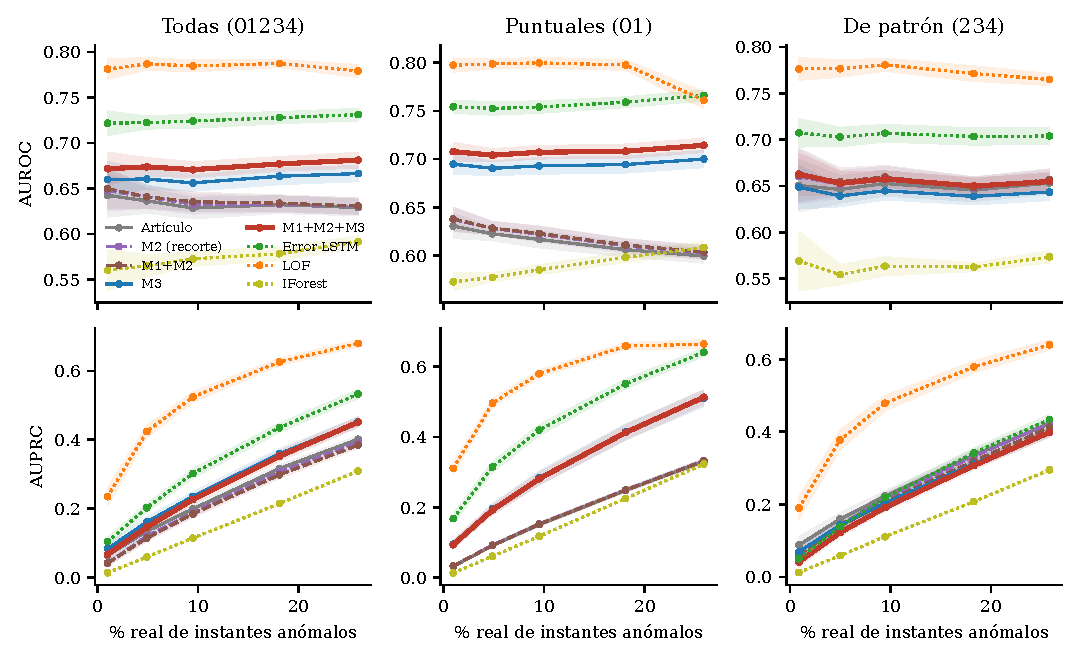
\includegraphics[width=\linewidth]{contaminacion_semi}
\caption{Contaminación semisintética sobre fondo real SMD: AUROC (arriba) y AUPRC (abajo) frente a la
proporción real de anomalías, por mezcla (10 máquinas $\times$ 3 semillas; bandas IC\,95\,\%).}
\label{fig:semi}
\end{figure}
